\documentclass[a4paper,landscape,9pt]{article}

\usepackage[margin=1cm]{geometry}
\usepackage{fontspec}
\setmainfont{TeX Gyre Pagella}
\usepackage{unicode-math}
\setmathfont{TeX Gyre Pagella Math}

\usepackage{tikz}
\usetikzlibrary{arrows.meta,calc,positioning,shapes.geometric}
\usepackage{microtype}

\pagestyle{empty}
\setlength{\parindent}{0pt}
\setlength{\parskip}{0.25em}

\tikzset{
  node-d/.style={draw,fill=black,regular polygon,regular polygon sides=6,minimum size=7mm,inner sep=0pt,text=white,font=\tiny\bfseries},
  node-a/.style={draw,fill=black!70,regular polygon,regular polygon sides=3,minimum size=7mm,inner sep=0pt,text=white,font=\tiny\bfseries},
  node-t/.style={draw,circle,minimum size=7mm,inner sep=0pt,line width=0.4pt,font=\tiny},
  node-o/.style={draw,fill=black!15,rectangle,minimum size=7mm,inner sep=0pt,font=\tiny},
  node-i/.style={draw,diamond,minimum size=8mm,inner sep=0pt,line width=0.4pt,font=\tiny},
  impl/.style={-{Latex[length=1.2mm]},line width=0.3pt,black!80},
  exemp/.style={-{Latex[length=1.2mm]},line width=0.3pt,dashed,black!80},
  band/.style={font=\scriptsize\scshape,text=black!60},
  bandline/.style={draw,black!18,line width=0.3pt},
}

\begin{document}

\begin{center}
{\large\scshape Proposisjonsgraf, seksjon 6}\hspace{0.8em}{\itshape Forma oppstår i feltet mellom agentar}
\end{center}

\vspace{-0.6em}

\begin{center}
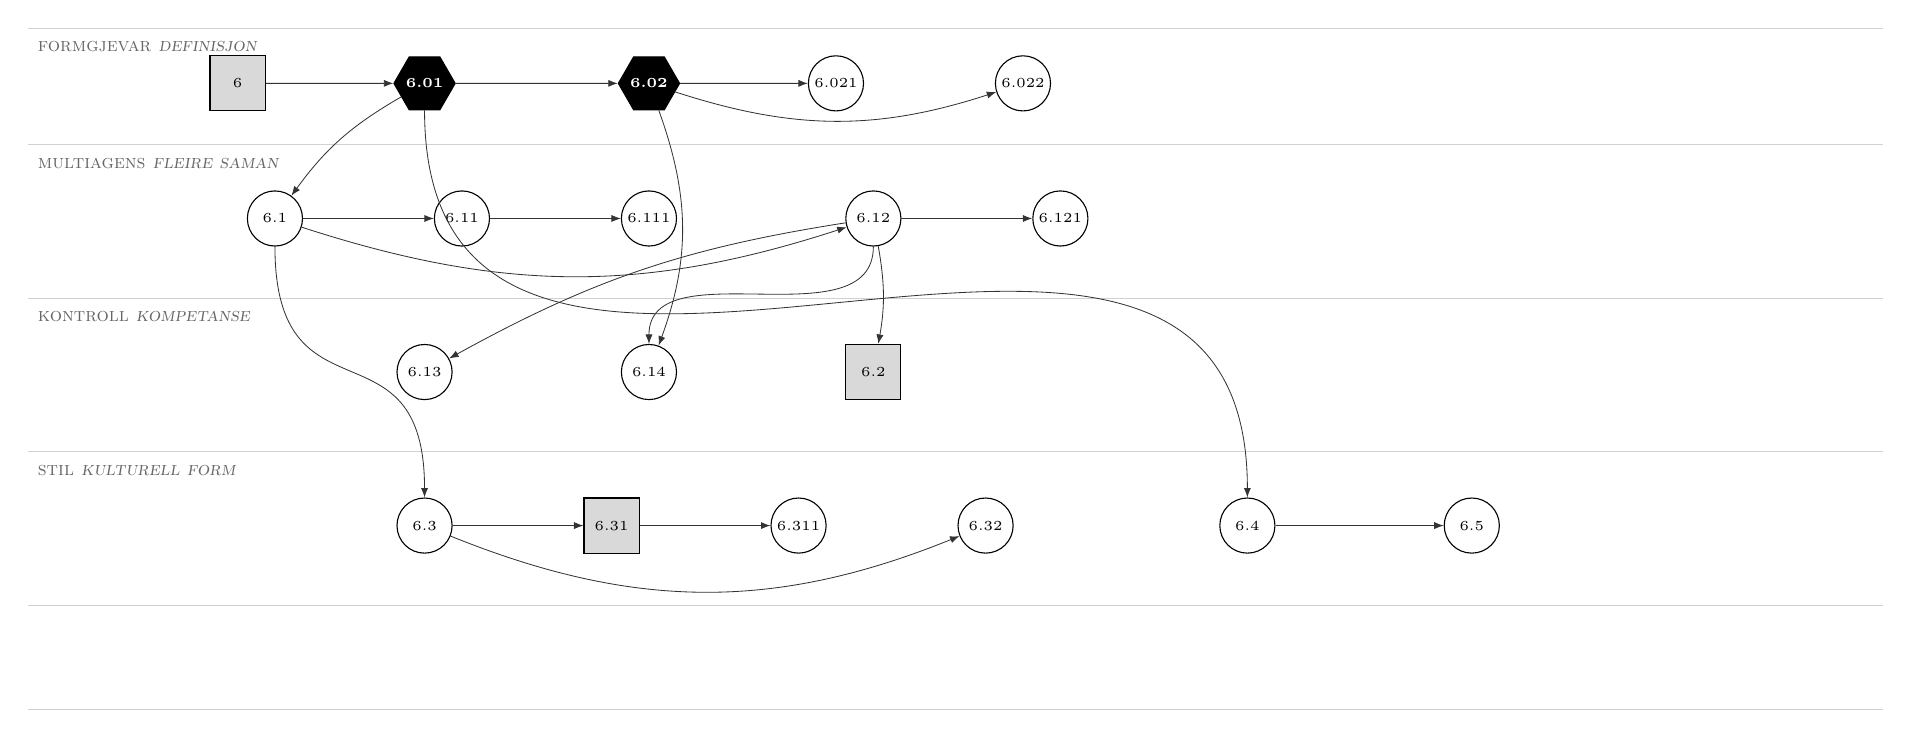
\begin{tikzpicture}[x=0.95cm,y=0.78cm]

  \draw[bandline] (-0.3, 0.6)  -- (24.5, 0.6);
  \draw[bandline] (-0.3, -1.3) -- (24.5, -1.3);
  \draw[bandline] (-0.3, -3.8) -- (24.5, -3.8);
  \draw[bandline] (-0.3, -6.3) -- (24.5, -6.3);
  \draw[bandline] (-0.3, -8.8) -- (24.5, -8.8);
  \draw[bandline] (-0.3, -10.5)-- (24.5, -10.5);

  \node[band,anchor=west] at (-0.3, 0.3)  {formgjevar  \itshape definisjon};
  \node[band,anchor=west] at (-0.3, -1.6) {multiagens  \itshape fleire saman};
  \node[band,anchor=west] at (-0.3, -4.1) {kontroll  \itshape kompetanse};
  \node[band,anchor=west] at (-0.3, -6.6) {stil  \itshape kulturell form};

  % BAND 1: formgjevar (definisjonskaskade)
  \node[node-o] (p6)     at (2.5, -0.3)  {6};
  \node[node-d] (p601)   at (5, -0.3)    {6.01};
  \node[node-d] (p602)   at (8, -0.3)    {6.02};
  \node[node-t] (p6021)  at (10.5, -0.3) {6.021};
  \node[node-t] (p6022)  at (13, -0.3)   {6.022};
  \draw[impl] (p6)   -- (p601);
  \draw[impl] (p601) -- (p602);
  \draw[impl] (p602) -- (p6021);
  \draw[impl] (p602) to[bend right=18] (p6022);

  % BAND 2: multiagens
  \node[node-t] (p61)    at (3, -2.5)    {6.1};
  \node[node-t] (p611)   at (5.5, -2.5)  {6.11};
  \node[node-t] (p6111)  at (8, -2.5)    {6.111};
  \node[node-t] (p612)   at (11, -2.5)   {6.12};
  \node[node-t] (p6121)  at (13.5, -2.5) {6.121};
  \draw[impl] (p601) to[bend right=12] (p61);
  \draw[impl] (p61)  -- (p611);
  \draw[impl] (p611) -- (p6111);
  \draw[impl] (p61)  to[bend right=18] (p612);
  \draw[impl] (p612) -- (p6121);

  % BAND 3: kontroll og kompetanse
  \node[node-t] (p613a)  at (5, -5)      {6.13};
  \node[node-t] (p614)   at (8, -5)      {6.14};
  \node[node-o] (p62)    at (11, -5)     {6.2};
  \draw[impl] (p612) to[bend right=10] (p613a);
  \draw[impl] (p602) to[bend left=20,looseness=1.0] (p614);
  \draw[impl] (p612) to[out=-90,in=90] (p614);
  \draw[impl] (p612) to[bend left=10] (p62);

  % BAND 4: stil og form (kulturelle konsekvensar)
  \node[node-t] (p63)    at (5, -7.5)    {6.3};
  \node[node-o] (p631)   at (7.5, -7.5)  {6.31};
  \node[node-t] (p6311)  at (10, -7.5)   {6.311};
  \node[node-t] (p632)   at (12.5, -7.5) {6.32};
  \node[node-t] (p64)    at (16, -7.5)   {6.4};
  \node[node-t] (p65)    at (19, -7.5)   {6.5};
  \draw[impl] (p61)  to[out=-90,in=90,looseness=1.6] (p63);
  \draw[impl] (p63)  -- (p631);
  \draw[impl] (p631) -- (p6311);
  \draw[impl] (p63)  to[bend right=22] (p632);
  \draw[impl] (p601) to[out=-90,in=90,looseness=1.3] (p64);
  \draw[impl] (p64)  -- (p65);

\end{tikzpicture}
\end{center}

\vspace{-0.2em}

\hrule

\vspace{0.4em}

\begin{minipage}[t]{0.325\textwidth}
{\scshape\small Lesing ovanfrå}

Rota \emph{6} seier at forma oppstår i feltet mellom agentar. Band 1 er traktaten sin didaktiske skarpe stad: \emph{6.01} definerer \textbf{formgjevar} som den generelle navigatøren, og \emph{6.02} definerer \textbf{designar} som den spesielle underklassen som navigerer på vegne av andre. \emph{6.021} og \emph{6.022} utfaldar den avgjerande asymmetrien: alle designarar er formgjevarar, men ikkje alle formgjevarar er designarar, og designaren har kapasitet til å nekte navigasjonen.

Band 2 løfter eit nivå opp: multiagens. \emph{6.1} seier at forma er eit poly-agentisk kompromiss, og \emph{6.12} at agens er multiskalar.
\end{minipage}\hfill
\begin{minipage}[t]{0.325\textwidth}
{\scshape\small Lesing nedover}

Band 3 skildrar kontrollstrukturen. \emph{6.13} seier at kontrollen alltid er delt: agenten vel, landskapet filtrerer. \emph{6.14} er eit konfluenspunkt: han har to foreldre, \emph{6.02} (designarens kapasitet) og \emph{6.12} (multiskalar agens). Saman er designaren aldri åleine i landskapet. \emph{6.2} observerer at tett samanbinding etablerer globale sløyfer og lar heilskapen sjølv bli agent.

Band 4 handsamar stil som kulturell form. \emph{6.3} er traktaten sin skarpaste stil-kritikk: stilarten manglar kausal kraft. \emph{6.31} observerer at stilen for brukaren er eit grensesnitt, ikkje eit symptom. \emph{6.4} og \emph{6.5} bind saman: kvar realisering utvidar det kjende, og inga form er endeleg.
\end{minipage}\hfill
\begin{minipage}[t]{0.325\textwidth}
{\scshape\small Strukturelle innsikter}

\emph{Konfluensen er attende.} Hypotesa styrkast: oppfinningseksjonar har konfluens. \emph{6.14} har to foreldre (designarens kapasitet og multiskalar agens). Dette er seksjonens syntesepunkt.

\emph{Ingen postulat.} Overraskande for ein oppfinningseksjon. Seksjon 5 hadde allereie etablert den postulative grunnen (agens eksisterer); seksjon 6 treng berre å utvida.

\emph{To definisjonar i lag.} \emph{6.01} og \emph{6.02} står side om side i band 1. Det er her traktaten gjev faget sin ryggrad: skiljet mellom formgjevar og designar.

\emph{6.3 som parallell til 2.21.} Begge reanalyserer stil-omgrepet. Seksjon 2 seier stil er eit aggregat; seksjon 6 seier stil manglar kausal kraft. Saman dannar dei traktaten sin samla kritikk av stil som årsak.

\emph{Statistisk profil.} To definisjonar, null postulat, to observasjonar, femten teorem. Oppfinning med låg risiko; seksjonen utfaldar det allereie etablerte.
\end{minipage}

\end{document}
